\chapter{Equazioni differenziali ordinarie}

\section{Richiami teorici}
	
	\noindent Il \emph{problema di Cauchy} consiste nel determinare una funzione \(y\) tale che
	\begin{equation}\label{eq:problema-cauchy}
		\begin{cases}
			y' (x) = f (x, y(x)) & x \ge x_0 \\
			y (x_0) = y_0
		\end{cases}
	\end{equation}
	con \(f \colon \varOmega \to \R^n\), ove \(\varOmega \subseteq \R \times \R^n\), e \((x_0, y_0) \in \varOmega\). In seguito supporremo che tale problema abbia un'unica soluzione.
	
	\begin{esempio}[Equazione differenziale ordinaria]
		Trovare \(y\) tale che
		\begin{equation*}
			\begin{cases}
				y' (x) = y (x) & x \ge 0 \\
				y (0) = 1
			\end{cases}
		\end{equation*}
		è un problema di Cauchy con \(f (x, y(x)) = y (x)\) e soluzione \(y (x) = \ee^x\).
	\end{esempio}

	\begin{esempio}[Sistema di equazioni differenziali ordinarie]
		Il sistema
		\begin{equation*}
			\begin{cases}
				y_1'(x) = - y_2 (x) & x \ge 0 \\
				y_2' (x) = y_1 (x) & x \ge 0 \\
				y_1 (0) = 1 \\
				y_2 (0) = 0
			\end{cases}
		\end{equation*}
		la cui soluzione è \(y (x) = (y_1 (x), y_2 (x)) = (\cos x, \sin x)\), è un problema di Cauchy con \(f (x, y (x)) = (- y_2 (x), y_1 (x))\).
	\end{esempio}

	\begin{teorema}[Picard-Lindelöf]\label{th:picard-lindelof}
		Definito \(D = [\, t_0 - \varepsilon, t_0 + \varepsilon \,] \times \R^n\) e considerato il problema
		\begin{equation*}
			\begin{cases}
				y' (t) = f (t, y(t)) & t \in [\, t_0 - \varepsilon, t_0 + \varepsilon \,] \\
				y (t_0) = y_0
			\end{cases}
		\end{equation*}
		se \(f \colon D \to \R\) è una funzione lipschitziana in \(y\), cioè esiste \(K \ge 0\) tale che
		\begin{equation*}
			\abs{f (t, \vec{y}_1) - f(t, \vec{y}_2)} \le K \norm{\vec{y}_1 - \vec{y}_2}
		\end{equation*}
		per ogni \((t, \vec{y}_1), (t, \vec{y}_2) \in D\), e continua in \(t\), allora esiste un'unica soluzione \(y\) al problema sull'intervallo \([\, t_0 - \varepsilon, t_0 + \varepsilon \,]\).
	\end{teorema}

	\begin{teorema}[Cauchy in piccolo]\label{th:cauchy-locale}
		Dato un aperto connesso \(D \subseteq \R \times \R^n\), siano \(f \colon D \to \R\) una funzione continua in \(D\) e \((t_0, \vec{y}_0)\) un punto interno di \(D\). Se \(f\) è lipschitziana nella seconda variabile, allora esiste un'unica funzione \(\vec{y}\) definita in un intervallo \([\, t_0 - \alpha, t_0 + \alpha \,]\), con \(\alpha > 0\), tale che
		\begin{equation*}
			\begin{cases}
				\vec{y}' (t) = f (t, \vec{y} (t)) & t \in [\, t_0 - \alpha, t_0 + \alpha \,] \\
				\vec{y} (t_0) = \vec{y}_0
			\end{cases}
		\end{equation*}
	\end{teorema}

	\begin{teorema}[Cauchy in grande]\label{th:cauchy-globale}
		Se \(f \colon [\, a, b \,] \times \R^n \to \R\) è continua nella prima variabile e lipschitziana nella seconda variabile, allora il problema di Cauchy
		\begin{equation*}
			\begin{cases}
				\vec{y}' (t) = f (t, \vec{y} (t)) & t \in [\, a, b \,] \\
				\vec{y} (a) = \vec{y}_0
			\end{cases}
		\end{equation*}
		ammette una e una sola soluzione \(\vec{y}\) definita su \([\, a, b \,]\) per ogni \(\vec{y}_0 \in \R^n\).
	\end{teorema}

	I Teoremi~\ref{th:cauchy-locale} e \ref{th:cauchy-globale} costituiscono teoremi di esistenza e unicità rispettivamente locale e globale.
	
	\begin{nota}
		Esistono problemi di Cauchy con soluzioni multiple. Il problema
		\begin{equation*}
			\begin{cases}
				y' (x) = 2 \sqrt{y (x)} & x > 0 \\
				y (x_0) = 0
			\end{cases}
		\end{equation*}
		ad esempio, ha come soluzioni
		\begin{equation*}
			y (x) =
			\begin{cases}
				(x - \alpha)^2 & x \ge \alpha \\
				0 & x < \alpha
			\end{cases}
		\end{equation*}
		al variare di \(\alpha \in \R_{> 0}\).
	\end{nota}

\section{Metodi numerici di risoluzione}
	
	\noindent Indicato con \(\intervallo (x, \bar{x})\) l'intervallo aperto che ha per estremi \(x\) e \(\bar{x}\), ossia \((\, x, \bar{x} \,)\) se \(x < \bar{x}\) o \((\, \bar{x}, x \,)\) se \(\bar{x} < x\), se si suppone che la soluzione al problema in \eqref{eq:problema-cauchy} sia sufficientemente regolare, allora dalla formula di Taylor segue che esiste \(\xi \in \intervallo (x, \bar{x})\) tale che
	\begin{equation*}
		\begin{split}
			y (x) &= y (\bar{x}) + y' (\bar{x}) (x - \bar{x}) + \frac{y'' (\xi)}{2} (x - \bar{x})^2 \\
			& \approx y (\bar{x}) + y' (\bar{x}) (x - \bar{x}) = y (\bar{x}) + f(\bar{x}, y (\bar{x})) (x - \bar{x})
		\end{split}
	\end{equation*}
	o, piú sinteticamente,
	\begin{equation}\label{eq:approx-prob-cauchy}
		y (x) \approx y (\bar{x}) + f (\bar{x}, y (\bar{x})) (x - \bar{x})
	\end{equation}
	
	Supponiamo ora di voler determinare un'approssimazione della soluzione nei punti equispaziati \(x_k = x_0 + k h\), ove \(x_0 \in \R\) e \(h > 0\) sono fissati -- equivalentemente si possono definire tali punti per ricorrenza: \(x_{k + 1} = x_k + h\) e \(x_0 \in \R\) fissato.
	
	\begin{definizione}\label{def:metodo-eulero-espl}
		Il \emph{metodo di Eulero esplicito} consiste nell'approssimare la soluzione \(y (x_k)\) con \(u_k\) secondo la formula
		\begin{align}\label{eq:metodo-eulero-espl}
			u_0 &= y (x_0) &
			u_{k + 1} &= u_k + h f (x_k, u_k)
		\end{align}
		che si ottiene dalla \eqref{eq:approx-prob-cauchy} effettuando la sostituzione \(x = x_{k + 1}\), \(\bar{x} = x_k\).
	\end{definizione}
	
	\begin{definizione}\label{def:metodo-eulero-impl}
		Il \emph{metodo di Eulero implicito} consiste nell'approssimare la soluzione \(y (x_k)\) con \(u_k\) secondo la formula
		\begin{align}\label{eq:metodo-eulero-impl}
			u_0 &= y (x_0) &
			u_{k + 1} &= u_k + h f (x_{k + 1}, u_{k + 1})
		\end{align}
		che si ottiene dalla \eqref{eq:approx-prob-cauchy} effettuando la sostituzione \(x = x_k\), \(\bar{x} = x_{k + 1}\).
	\end{definizione}
	
	\begin{osservazione}
		Ogni iterazione del metodo di Eulero implicito richiede la risoluzione di un'equazione non lineare nell'incognita \(z\) del tipo \(z = u_k + h f(x_{k + 1}, z)\). La soluzione di quest'equazione può essere calcolata ricorrendo a metodi quali il metodo di Newton, il metodo di punto fisso o il metodo delle secanti.
	\end{osservazione}

	\begin{osservazione}
		Indipendentemente dalla derivazione dovuta alla formula di Taylor, i metodi di Eulero esplicito ed Eulero implicito possono essere utilizzati anche per approssimare funzioni \(y\) a valori in \(\R^n\) con \(n > 1\).
	\end{osservazione}

	\begin{definizione}\label{def:metodo-lm}
		Un \emph{metodo \inglese{linear multistep}} consiste nell'approssimare la soluzione \(y (x_k)\) con \(u_k\) secondo la formula
		\begin{align}\label{eq:metodo-lm}
			u_0 &= y (x_0) &
			u_{k + 1} &= \sum_{j = 0}^p a_j u_{k - j} + h \sum_{j = - 1}^p b_j f (x_{k - j}, u_{k - j})
		\end{align}
	\end{definizione}

	\begin{osservazione}
		I metodi \inglese{linear multistep} necessitano di \(u_{n - p}, \dots, u_n\) per calcolare \(u_{n + 1}\); per questo motivo sono chiamati \emph{metodi a \(p + 1\) passi}. Dal momento che all'inizio si dispone solo di \(u_0\) e un metodo \inglese{linear multistep} necessiterebbe anche di \(u_1, \dots, u_p\), per ottenere questi ultimi si ricorre ad altre strategie, come ad esempio applicare piú volte metodi ad un passo quali Eulero esplicito.
		
		Si noti, poi, che il metodo è esplicito se \(b_{- 1} = 0\), implicito altrimenti.
	\end{osservazione}
	
	\begin{osservazione}
		I metodi di Eulero esplicito ed Eulero implicito sono metodi \inglese{linear multistep}: è sufficiente, infatti, porre nella \eqref{eq:metodo-lm}
		\begin{itemize}
			\item Eulero esplicito: \(p = 0\), \(a_0 = 1\), \(b_{- 1} = 0\), \(b_0 = 1\);
			\item Eulero implicito: \(p = 0\), \(a_0 = 1\), \(b_{- 1} = 1\), \(b_0 = 0\).
		\end{itemize}
	\end{osservazione}

	Dovendo studiare il problema di Cauchy in \eqref{eq:problema-cauchy} e volendo approssimare la sua soluzione \(y\) nei punti equispaziati \(x_k = x_0 + k h\), osserviamo che
	\begin{equation*}
		y (x_{n + k}) = y (x_{n - j}) + \int_{x_{n - j}}^{\mathrlap{x_{n + k}}} y' (t) \dd{t} = y (x_{n - j}) + \int_{x_{n - j}}^{\mathrlap{x_{n + k}}} f (t, y (t)) \dd{t}
	\end{equation*}
	Se si sostituisce l'integranda col polinomio di grado al piú \(p\)
	\begin{equation*}
		\pi_p (x) = \sum_{i = 0}^p f (x_{n - i}, y (x_{n - i})) \, L_i (x)
	\end{equation*}
	che interpola le coppie \((x_\ell, f(x_\ell, y (x_\ell)))\) per \(\ell \in \Set{n - p, \dots, n}\), ove \(L_i (x)\) è l'\(i\)-esimo polinomio di Lagrange definito nella \eqref{eq:polin-lagrange}, si ricava, posto
	\begin{equation}\label{eq:metodo-lm-beta}
		\beta_{p, i}^{(k, j)} = \frac{1}{h} \int_{x_{n - j}}^{\mathrlap{x_{n + k}}} L_i (t) \dd{t} = \int_{- j}^k \prod_{\substack{m = 0 \\ m \ne i}}^p \frac{s + m}{-i + m} \dd{s}
	\end{equation}
	per ogni \(i \in \Set{0, \dots, p}\), un metodo \inglese{linear multistep} a piú passi
	\begin{equation}\label{eq:metodo-lm-con-integrale}
		\begin{split}
			y (x_{n + k}) &= y (x_{n - j}) + \int_{x_{n - j}}^{\mathrlap{x_{n + k}}} f (t, y (t)) \dd{t} \\
			&\approx y (x_{n - j}) + \int_{x_{n - j}}^{x_{n + k}} \sum_{i = 0}^p f (x_{n - i}, y (x_{n - i})) \, L_i (t) \dd{t} \\
			&= y (x_{n - j}) + \sum_{i = 0}^p f (x_{n - i}, y (x_{n - i})) \int_{x_{n - j}}^{\mathrlap{x_{n + k}}} L_i (t) \dd{t} \\
			&= y (x_{n - j}) + h \sum_{i = 0}^p \beta_{p, i}^{(k, j)} f (x_{n - i}, y (x_{n - i}))
		\end{split}
	\end{equation}

	\begin{esempio}[Metodi di Adams-Bashforth]
		Ponendo \(k = 1\) e \(j = 0\) nella \eqref{eq:metodo-lm-con-integrale}, si ottiene la famiglia di metodi espliciti di Adams-Bashforth. Tra questi metodi ci sono i seguenti, tutti a \(p + 1\) passi, ove si è posto \(f_k = f (x_k, y (x_k))\):
		\begin{itemize}
			\item \(p = 0\): \(u_{n + 1} = u_n + h f_n\) (metodo di Eulero esplicito);
			\item \(p = 1\): \(u_{n + 1} = u_n + \frac{h}{2} (3 f_n - f_{n - 1})\);
			\item \(p = 2\): \(u_{n + 1} = u_n + \frac{h}{12} (23 f_n - 16 f_{n - 1} + 5 f_{n - 2})\);
			\item \(p = 3\): \(u_{n + 1} = u_n + \frac{h}{24} (55 f_n - 59 f_{n - 1} + 37 f_{n - 2} - 9 f_{n - 3})\).
		\end{itemize}
	\end{esempio}

	\begin{esempio}[Metodi di Adams-Moulton]
		Ponendo \(k = 0\) e \(j = 1\) nella \eqref{eq:metodo-lm-con-integrale}, si ottiene la famiglia di metodi impliciti di Adams-Moulton. Tra questi metodi ci sono i seguenti, ove si è posto \(f_k = f (x_k, y (x_k))\):
		\begin{itemize}
			\item \(p = 0\): \(u_{n + 1} = u_n + h f_{n + 1}\) (metodo di Eulero implicito);
			\item \(p = 1\): \(u_{n + 1} = u_n + \frac{h}{2} (f_{n + 1} + f_n)\) (metodo di Crank-Nicolson);
			\item \(p = 2\): \(u_{n + 1} = u_n + \frac{h}{12} (5 f_{n + 1} + 8 f_n - f_{n - 1})\);
			\item \(p = 3\): \(u_{n + 1} = u_n + \frac{h}{24} (9 f_{n + 1} + 19 f_n - 5 f_{n - 1} + f_{n - 2})\).
		\end{itemize}
	\end{esempio}

	Si verifica facilmente che sia i metodi di Adams-Bashforth sia quelli di Adams-Moulton sono metodi \inglese{linear multistep}.
	
	\begin{esempio}[Metodi di Nyström]
		Ponendo \(k = 1\) e \(j = 1\) nella \eqref{eq:metodo-lm-con-integrale}, si ottiene la famiglia di metodi di Nyström. Tra questi metodi c'è il metodo del punto medio \(u_{n + 1} = u_{n - 1} + 2 h f_n\), ove si è posto \(f_n = f (x_n, y (x_n))\).
	\end{esempio}

	Un altro esempio di metodo derivato dalla \eqref{eq:metodo-lm-con-integrale} è quello di Milne \(u_{n + 1} = u_{n - 1} + \frac{h}{3} (f_{n - 1} + 4 f_n + f_{n + 1})\), ottenuto ponendo \(k = 0\), \(j = 2\) e \(p = 2\).
	
\section[Consistenza dei metodi \textsc{lm}]{Consistenza dei metodi LM}
	
	\begin{definizione}[Errore di troncamento]
		Dovendo risolvere un problema di Cauchy come in \eqref{eq:problema-cauchy} nel compatto \([\, x_0, b \,]\) tramite un metodo \inglese{linear multistep} come nella \eqref{eq:metodo-lm}, chiamati \(y\) la soluzione di \eqref{eq:problema-cauchy} e \(x_k = x_0 + k h\) punti equispaziati per \(k \in \Set{0, \dots, N}\) tali che \(b - h < x_N \le b\), si dice \emph{errore locale di troncamento} del metodo la quantità
		\begin{equation}\label{eq:err-loc-tronc}
			\tau_n (h) = \frac{1}{h} \qty[y (x_{n + 1}) - \qty(\sum_{j = 0}^p a_j y (x_{n - j}) + h \sum_{\mathclap{j = - 1}}^p b_j f (x_{n - j}, y (x_{n - j})))]
		\end{equation}
		Supposto che sia stato commesso errore nullo nei passi iniziali, si dice \emph{errore globale di troncamento} del metodo la quantità
		\begin{equation}\label{eq:err-glob-tronc}
			\tau (h) = \max \Set{\abs{\tau_n (h)} : n \in \Set{0, \dots, N}}
		\end{equation}
	
		Un metodo tale che \(\tau (h) \xrightarrow{h \to 0} 0\) si dice \emph{consistente}. Se \(\tau (h) = \order{h^k}\) quando \(h \to 0\), si dice che il metodo ha \emph{ordine di consistenza} \(k\).
	\end{definizione}

	La consistenza è un indice di quanto la soluzione del problema \eqref{eq:problema-cauchy} verifichi lo schema discreto del metodo \inglese{linear multistep} \eqref{eq:metodo-lm}. Per metodi espliciti, poi, la quantità detta \emph{residuo}
	\begin{equation*}
		y (x_{n + 1}) - \qty(\sum_{j = 0}^p a_j y (x_{n - j}) + h \sum_{\mathclap{j = - 1}}^p b_j f (x_{n - j}, y (x_{n - j})))
	\end{equation*}
	corrisponde all'errore dello schema discreto se \(u_{n - j} = y (x_{n - j})\) per ogni \(j \in \Set{0, \dots, p}\).
	
	\begin{teorema}[Errore locale di troncamento del metodo di Eulero esplicito]\label{th:metodo-eulero-espl-consist}
		Se l'unica soluzione \(y\) al problema \eqref{eq:problema-cauchy} in \([\, a, b \,]\) è di classe \(\cont^2 ([\, a, b \,])\) e si definiscono \(x_k = a + k h\) per \(k \in \Set{0, \dots, N}\) con \(b - h < x_N \le b\), allora per ogni \(k \in \Set{0, \dots, N - 1}\) esiste \(\xi_k \in (\, x_k, x_{k + 1} \,)\) tale che il metodo di Eulero esplicito verifichi
		\begin{equation}\label{eq:metodo-eulero-espl-consist}
			\tau_k (h) = \frac{y'' (\xi_k)}{2} h
		\end{equation}
	\end{teorema}

	\begin{proof}
		Dalla formula di Taylor si ottiene
		\begin{equation*}
			y (x_{k + 1}) = y (x_k) + y' (x_k) (x_{k + 1} - x_k) + \frac{y'' (\xi_k)}{2} (x_{k + 1} - x_k)^2
		\end{equation*}
		per un certo \(\xi_k \in (\, x_k, x_{k + 1} \,)\); dato che \(x_{k + 1} - x_k = h\), segue che
		\begin{equation*}
			y (x_{k + 1}) - y (x_k) - h f (x_k, y (x_k)) = \frac{y'' (\xi_k)}{2} h^2
		\end{equation*}
		e, quindi,
		\begin{equation*}
			\begin{split}
				\tau_k (h) &= \frac{1}{h} \qty[y (x_{k + 1}) - y (x_k) - h f (x_k, y (x_k))] \\
				&= \frac{1}{h} \qty(\frac{y'' (\xi_k)}{2} h^2) = \frac{y'' (\xi_k)}{2} h \qedhere
			\end{split}
		\end{equation*}
	\end{proof}

	\begin{osservazione}
		In base al Teorema~\ref{th:metodo-eulero-espl-consist}, se \(y \in \cont^2 ([\, a, b \,])\), allora
		\begin{equation*}
			M = \max_{x \in [\, a, b \,]} \abs{y'' (x)} \implies \tau (h) = \max_{n \in \Set{0, \dots, N}} \abs{\frac{y'' (\xi_n)}{2} h} \le \frac{M h}{2}
		\end{equation*}
		ossia il metodo di Eulero esplicito è consistente e ha ordine di consistenza \(1\).
	\end{osservazione}

	\begin{teorema}[Errore locale di troncamento del metodo di Eulero implicito]\label{th:metodo-eulero-impl-consist}
		Se l'unica soluzione \(y\) al problema \eqref{eq:problema-cauchy} in \([\, a, b \,]\) è di classe \(\cont^2 ([\, a, b \,])\) e si definiscono \(x_k = a + k h\) per \(k \in \Set{0, \dots, N}\) con \(b - h < x_N \le b\), allora per ogni \(k \in \Set{0, \dots, N - 1}\) esiste \(\xi_k \in (\, x_k, x_{k + 1} \,)\) tale che il metodo di Eulero implicito verifichi
		\begin{equation}\label{eq:metodo-eulero-impl-consist}
			\tau_k (h) = - \frac{y'' (\xi_k)}{2} h
		\end{equation}
	\end{teorema}

	\begin{proof}
		Dalla formula di Taylor si ottiene
		\begin{equation*}
			y (x_k) = y (x_{k + 1}) + y' (x_{k + 1}) (x_k - x_{k + 1}) + \frac{y'' (\xi_k)}{2} (x_k - x_{k + 1})^2
		\end{equation*}
		per un certo \(\xi_k \in (\, x_k, x_{k + 1} \,)\); dato che \(x_{k + 1} - x_k = h\), segue che
		\begin{equation*}
			y (x_{k + 1}) - y (x_k) - h f (x_{k + 1}, y (x_{k + 1})) = - \frac{y'' (\xi_k)}{2} h^2
		\end{equation*}
		e, quindi,
		\begin{equation*}
			\begin{split}
				\tau_k (h) &= \frac{1}{h} \qty[y (x_{k + 1}) - y (x_{k + 1}) - h f (x_{k + 1}, y (x_{k + 1}))] \\
				&= \frac{1}{h} \qty(- \frac{y'' (\xi_k)}{2} h^2) = - \frac{y'' (\xi_k)}{2} h \qedhere
			\end{split}
		\end{equation*}
	\end{proof}

	\begin{osservazione}
		In base al Teorema~\ref{th:metodo-eulero-impl-consist}, se \(y \in \cont^2 ([\, a, b \,])\), allora
		\begin{equation*}
			M = \max_{x \in [\, a, b \,]} \abs{y'' (x)} \implies \tau (h) = \max_{n \in \Set{0, \dots, N}} \abs{- \frac{y'' (\xi_n)}{2} h} \le \frac{M h}{2}
		\end{equation*}
		ossia il metodo di Eulero implicito è consistente e ha ordine di consistenza \(1\).
	\end{osservazione}

	\begin{teorema}\label{th:metodo-lm-consistenza}
		Un metodo \inglese{linear multistep} è consistente se e solo se
		\begin{subequations}\label{eq:metodo-lm-consistenza}
			\begin{gather}
				\sum_{j = 0}^p a_j = 1 \\
				- \sum_{j = 0}^p j a_j + \sum_{j = - 1}^p b_j = 1
			\end{gather}
		\end{subequations}
		
		Se la soluzione \(y\) a \eqref{eq:problema-cauchy} è di classe \(\cont^{q + 1}\) per \(q \ge 1\), un metodo \inglese{linear multistep} ha ordine di consistenza \(q\) se e solo se è consistente e per ogni \(i \in \Set{2, \dots, q}\)
		\begin{equation}\label{eq:metodo-lm-consistenza-q}
			\sum_{j = 0}^p (-j)^i a_j + i \sum_{j = - 1}^p (-j)^{i - 1} b_j = 1
		\end{equation}
	\end{teorema}

	\begin{esempio}
		Il metodo di Eulero esplicito ha parametri \(a_0 = 1\), \(b_{- 1} = 0\), \(b_0 = 1\) e \(p = 0\); è immediato vedere che vale la \eqref{eq:metodo-lm-consistenza-q} con \(q = 1\), ossia che ha ordine di consistenza \(1\).
		
		Il metodo di Eulero implicito ha parametri \(a_0 = 1\), \(b_{- 1} = 1\), \(b_0 = 0\) e \(p = 0\); è immediato vedere che vale la \eqref{eq:metodo-lm-consistenza-q} con \(q = 1\), ossia che ha ordine di consistenza \(1\).
		
		Il metodo di Crank-Nicolson ha parametri \(a_0 = 1\), \(b_{- 1} = 1 / 2\), \(b_0 = 1 / 2\) e \(p = 0\); è immediato vedere che vale la \eqref{eq:metodo-lm-consistenza-q} con \(q = 1\), ossia che ha ordine di consistenza \(1\). Con un conto diretto, poi, si vede che la \eqref{eq:metodo-lm-consistenza-q} vale anche per \(i = 2\); se, quindi, \(y \in \cont^3 ([\, a, b \,])\), allora il metodo ha ordine di consistenza \(2\).
	\end{esempio}

\section[Stabilità dei metodi \textsc{lm}]{Stabilità dei metodi LM}
	
	\begin{definizione}[Zero-stabilità]\label{def:zero-stabile}
		Dovendo risolvere un problema del tipo \eqref{eq:problema-cauchy} nell'intervallo \([\, a, b \,]\) tramite un metodo \inglese{linear multistep} a \(p\) passi, si considerino i punti equispaziati \(x_k = a + k h_N\), con \(h_N = (b - a) / N\) e \(k \in \Set{0, \dots, N}\). Il metodo impiegato si dice \emph{zero-stabile} se, comunque scelte due successioni \(\bigl( u_k^{(h_N)} \bigr)_{k \in \N}\) e \(\bigl( v_k^{(h_N)} \bigr)_{k \in \N}\) generate dal metodo, indicati con \(u_0^{(h_N)}, \dots, u_{p - 1}^{(h_N)}\) e con \(v_0^{(h_N)}, \dots, v_{p - 1}^{(h_N)}\) rispettivamente i dati iniziali delle due successioni, esistono \(h^*, K > 0\) tali che per ogni \(h_N \le h^*\) si abbia
		\begin{equation}
			\max_{s \in \Set{0, \dots, N}} \abs{u_s^{(h_N)} - v_s^{(h_N)}} \le K \max_{s \in \Set{0, \dots, p - 1}} \abs{u_s^{(h_N)} - v_s^{(h_N)}}
		\end{equation}
	\end{definizione}

	Questa proprietà è chiamata zero-stabilità perché determinata soltanto dallo studio relativo al problema in \eqref{eq:problema-cauchy} con \(f (x, y) = 0\). Benché noi ci limitiamo allo studio dei \textsc{lmm}, esistono definizioni che permettono un'analisi analoga di altri metodi piú generali.
	
	In generale, è complicato studiare caso per caso la stabilità dei \textsc{lmm}, mentre risulta piú facile studiarne la \inglese{root condition}, che è un concetto equivalente: essa è soddisfatta se il polinomio caratteristico
	\begin{equation*}
		\varrho (z) = z^{p + 1} - \sum_{k = 0}^p a_k z^k
	\end{equation*}
	ha tutte le radici nella palla chiusa complessa \(\overline{B (0, 1)}\) e le radici in \(\partial B (0, 1)\) hanno molteplicità \(1\).
	
	\begin{esempio}
		Volendo analizzare la \inglese{root condition} dei metodi di Eulero esplicito, Eulero implicito e Crank-Nicolson, poiché \(a_0 = 1\) e \(p = 0\), il loro polinomio caratteristico è \(\varrho (z) = z - 1\), che ha come unica soluzione \(z^* = 1\); dato che questa soluzione è in \(\partial B (0, 1)\) con molteplicità \(1\), i tre metodi sono tutti zero-stabili.
	\end{esempio}

\section[Convergenza dei metodi \textsc{lm}]{Convergenza dei metodi LM}
	
	\begin{definizione}[Convergenza]
		Dovendo risolvere il problema di Cauchy \eqref{eq:problema-cauchy} nell'intervallo \([\, x_0, x_{\textup{fin}} \,]\), siano \(x_s = x_0 + s h_N\) per \(s \in \Set{0, \dots, N}\) con \(N h_N = x_{\textup{fin}} - x_0\), \(y^{(h_N)} = (y (x_0), \dots, y (x_N))\) la soluzione esatta di \eqref{eq:problema-cauchy} e \(u^{(h_N)} = (u_0, \dots, u_N)\) la \((N + 1)\)-upla di approssimazioni della soluzione fornite da un metodo \inglese{linear multistep} a \(p + 1\) passi. Tale metodo \inglese{linear multistep} si dice \emph{convergente} se, qualora i passi iniziali \(u_0^{(h_N)}, \dots, u_p^{(h_N)}\) verifichino
		\begin{subequations}
		\begin{equation}
			\eta (h_N) = \max_{k \in \Set{0, \dots, p}} \abs{y_k^{(h_N)} - u_k^{(h_N)}} \xrightarrow{h_N \to 0} 0
		\end{equation}
		si ha
		\begin{equation}
			\norm{y^{(h_N)} - u^{(h_N)}}_\infty \xrightarrow{h_N \to 0} 0
		\end{equation}
		\end{subequations}
	
		Il metodo si dice \emph{convergente con ordine \(q\)} se esistono \(C_1, C_2\) indipendenti da \(h_N\) tali che
		\begin{equation}
			\eta (h_N) \le C_1 h_N^q \implies \norm{y^{(h_N)} - u^{(h_N)}} \le C_2 h_N^q
		\end{equation}
	\end{definizione}

	\begin{osservazione}
		È possibile dimostrare che un metodo è convergente se e solo se è consistente e stabile. Di conseguenza, se un metodo verifica la \inglese{root condition} e le condizioni di consistenza, allora è convergente.
		
		In particolare, i metodi di Eulero esplicito ed Eulero implicito sono convergenti.
	\end{osservazione}

	\begin{esempio}\label{eg:eul-espl-prob-test}
		Si consideri il problema di Cauchy
		\begin{equation*}
			\begin{cases}
				y' (x) = y (x) & x \in [\, 0, 1 \,] \\
				y (0) = 1
			\end{cases}
		\end{equation*}
		che ha come soluzione \(y (x) = \ee^x\), e si applichi il metodo di Eulero esplicito per approssimare la soluzione nei punti \(x_k = k h_n\) ove \(k \in \Set{0, \dots, N_n}\) e \(h_n = 1 / N_n\); scelto come dato iniziale \(u_0 = 1 + h_n\), nella Figura~\ref{fig:eul-espl-prob-test} si riportano gli errori assoluti commessi dal metodo -- che sembra essere convergente.
		
		\begin{figure}[tpb]
			\centering
			
			\begin{tikzpicture}
				\begin{axis}[xlabel=\(x\), ylabel={Errore}, legend entries = {{\(N_1 = 8\)}, {\(N_2 = 16\)}, {\(N_3 = 32\)}, {\(N_4 = 64\)}, {\(N_5 = 128\)}}, legend pos = outer north east, legend cell align={left}]
					\addplot table {risorse/eulero08.dat};
					\addplot table {risorse/eulero16.dat};
					\addplot table {risorse/eulero32.dat};
					\addplot+[color = black!30!green] table {risorse/eulero64.dat};
					\addplot+[thick, color = blue!50!red, no marks] table {risorse/eulero128.dat};
				\end{axis}
			\end{tikzpicture}
		
			\caption{Rappresentazione degli errori del metodo di Eulero esplicito nell'approssimazione della soluzione del problema di Cauchy nell'Esempio~\ref{eg:eul-espl-prob-test}.}\label{fig:eul-espl-prob-test}
		\end{figure}
	\end{esempio}

	\begin{esempio}\label{eg:consist-prob-test}
		Si consideri il problema di Cauchy
		\begin{equation*}
			\begin{cases}
				y' (x) = y (x) & x \in [\, 0, 1 \,] \\
				y (0) = 1
			\end{cases}
		\end{equation*}
		che ha come soluzione \(y (x) = \ee^x\), e si applichi il metodo consistente
		\begin{equation*}
			u_{n + 2} = - 4 u_{n + 1} + 5 u_n + h_k \qty(4 f(x_{n + 1}, u_{n + 1}) + 2 f (x_n, u_n))
		\end{equation*}
		per approssimare la soluzione nei punti \(x_k = k h_n\) ove \(k \in \Set{0, \dots, N_n}\) e \(h_n = 1 / N_n\); scelti come dati iniziali \(u_0 = 1\) e \(u_1 = h_n\), nella Figura~\ref{fig:consist-prob-test} si riportano gli errori assoluti commessi dal metodo -- che non risulta convergente.
		
		\begin{figure}[tpb]
			\centering
			
			\begin{tikzpicture}
				\begin{axis}[xlabel=\(x\), ylabel={Errore}, legend entries = {{\(N_1 = 10\)}, {\(N_2 = 20\)}, {\(N_3 = 40\)}, {\(N_4 = 80\)}}, legend pos = outer north east, legend cell align={left}, ymode = log]
					\addplot table {risorse/consistente10.dat};
					\addplot table {risorse/consistente20.dat};
					\addplot table {risorse/consistente40.dat};
					\addplot+[color = black!30!green] table {risorse/consistente80.dat};
				\end{axis}
			\end{tikzpicture}
			
			\caption{Rappresentazione degli errori del metodo proposto nell'Esempio~\ref{eg:consist-prob-test} nell'approssimazione della soluzione del problema di Cauchy.}\label{fig:consist-prob-test}
		\end{figure}
	\end{esempio}

	\begin{teorema}\label{th:metodo-lm-convergenza}
		Dovendo studiare il problema di Cauchy \eqref{eq:problema-cauchy} nell'intervallo \([\, x_0, x_{\textup{fin}} \,]\), si supponga che \(f \colon [\, x_0, x_{\textup{fin}} \,] \times \R \to \R\) sia continua e \(L\)-lipschitziana rispetto alla seconda variabile e che la soluzione \(y\) sia di classe \(\cont^1\). Considerato un metodo \inglese{linear multistep} a \(p + 1\) passi, se 
		\begin{itemize}
			\item i dati iniziali verificano
			\begin{equation*}
				\eta (h) = \max_{i \in \Set{0, \dots, p}} \abs{y (x_i) - u_i} \xrightarrow{h \to 0} 0
			\end{equation*}
			\item il metodo è consistente;
			\item \(a_j \ge 0\) per ogni \(j \in \Set{0, \dots, p}\);
			\item \(h \le h^* = 1 / (2 c)\) con \(c = L \sum_{j = - 1}^p \abs{b_j}\);
		\end{itemize}
		allora il metodo \inglese{linear multistep} è convergente ed esistono \(C_1, C_2 > 0\) tali che per ogni \(n\)
		\begin{equation}
			\abs{y (x_n) - u_n} \le C_1 \eta (h) + C_2 \tau (h)
		\end{equation}
		
		Se \(y \in \cont^{m + 1} ([\, x_0, x_{\textup{fin}} \,])\), il metodo ha ordine di consistenza pari a \(m\) e gli errori iniziali soddisfano \(\eta (h) = \order{h^m}\), allora il metodo ha ordine di convergenza pari a \(m\).
	\end{teorema}

	\begin{osservazione}
		I metodi di Adams-Bashforth e Adams-Moulton presentati sono tutti consistenti con ordine \(p + 1\) e verificano \(a_0 = 1\), \(a_1 = \dots = a_p = 0\); dal momento che, poi, gli zeri del polinomio caratteristico \(z^{p + 1} - 1\) sono le radici \((p + 1)\)-esime dell'unità, ciascuna con molteplicità \(1\), tali metodi soddisfano la \inglese{root condition} e, quindi, sono convergenti.
		
		Se la soluzione \(y\) del problema in \eqref{eq:problema-cauchy} è di classe \(\cont^{p + 2}\), il metodo ha ordine di consistenza \(p + 1\) e gli errori iniziali soddisfano \(\eta (h) = \order{h^m}\), allora il metodo converge con ordine \(p + 1\).
		
		In particolare, nelle ipotesi del Teorema~\ref{th:metodo-lm-convergenza}, si ha quanto segue:
		\begin{itemize}
			\item il metodo di Eulero esplicito, che ha ordine di consistenza \(1\), è convergente con ordine di convergenza \(1\);
			\item il metodo di Eulero implicito, che ha ordine di consistenza \(1\), è convergente con ordine di convergenza \(1\);
			\item il metodo di Crank-Nicolson, che ha ordine di consistenza \(2\), è convergente con ordine di convergenza \(2\).
		\end{itemize}
	\end{osservazione}

\section[Assoluta stabilità dei metodi \textsc{lm}]{Assoluta stabilità dei metodi LM}
	
	\noindent Nello studio delle equazioni differenziali ordinarie, è interessante verificare diversi tipi di stabilità; noi studieremo la cosiddetta assoluta stabilità. Definito il problema di Cauchy
	\begin{equation}\label{eq:problema-cauchy-exp}
		\begin{cases}
			y' (x) = \lambda y(x) & x \ge 0 \\
			y (0) = 1
		\end{cases}
	\end{equation}
	ove \(\lambda \in \C\) tale che \(\Re \lambda \le 0\), che ha come soluzione \(y (x) = \exp(\lambda x)\), si cerca un passo \(h\) tale che il metodo numerico impiegato per risolvere il problema \eqref{eq:problema-cauchy} abbia lo stesso comportamento asintotico di \(\exp (\lambda x)\).
	
	Di un metodo numerico la \emph{regione di assoluta stabilità} consiste nell'insieme degli \(h \lambda\) tali che la soluzione approssimata da questo metodo abbia lo stesso comportamento asintotico della soluzione al problema in \eqref{eq:problema-cauchy-exp} relativo al parametro \(\lambda\) -- se \(\Re \lambda < 0\).
	
	\begin{subequations}
		In generale, determinare la soluzione del problema di Cauchy
		\begin{equation}\label{eq:prob-cauchy-generico}
			\begin{cases}
				y' (x) = f (x, y (x)) & x \ge 0 \\
				y (x_0) = y_0
			\end{cases}
		\end{equation}
		è complicato. È piú semplice, invece, risolvere
		\begin{equation}\label{eq:prob-cauchy-particolare}
			\begin{cases}
				y' (x) = \lambda y (x) + g (x) & x \ge 0 \\
				y (0) = y_0
			\end{cases}
		\end{equation}
		visto che esiste la formula risolutiva esplicita
		\begin{equation*}
			y (x) = y_0 \ee^{\lambda x} + \int_0^x \exp [\lambda (x - t)] g (t) \dd{t}
		\end{equation*}
		Chiamata \(y\) la soluzione al problema in \eqref{eq:prob-cauchy-particolare} e \(y_\varepsilon\) la soluzione del problema di Cauchy
		\begin{equation}\label{eq:prob-cauchy-perturbato}
			\begin{cases}
				y' (x) = \lambda y (x) + g (x) & x \ge 0 \\
				y (0) = y_0 + \varepsilon
			\end{cases}
		\end{equation}
		si vede che \(z_\varepsilon = y_\varepsilon - y\) risolve il problema di Cauchy
		\begin{equation}
			\begin{cases}
				z_\varepsilon' (x) = \lambda z_\varepsilon (x) & x \ge 0 \\
				z_\varepsilon (0) = \varepsilon
			\end{cases}
		\end{equation}
		che ha come soluzione \(z_\varepsilon (x) = \varepsilon \ee^{\lambda x}\).
	\end{subequations}

	Nelle applicazioni si suppone che \(\lambda < 0\) oppure che \(\Re \lambda < 0\) perché in questi casi \(z_\varepsilon (x) \xrightarrow{x \to + \infty} 0\) e, quindi, l'effetto delle perturbazioni si annulla per grandi valori di \(x\). Il fatto che anche il metodo numerico goda di queste proprietà spinge a studiare la regione di stabilità di tale metodo.
	
	\begin{definizione}
		Un problema di Cauchy come in \eqref{eq:problema-cauchy-exp} si dice \inglese{stiff} se \(\Re \lambda \ll 0\).
	\end{definizione}

	\begin{esempio}[Assoluta stabilità del metodo di Eulero esplicito]
		Volendo approssimare la soluzione di \eqref{eq:problema-cauchy-exp} col metodo di Eulero esplicito
		\begin{align*}
			u_0 &= 1 &
			u_n &= u_{n - 1} + h f (x_{n - 1}, u_{n - 1}) = (1 + h \lambda) u_{n - 1}
		\end{align*}
		iterando la definizione si vede che
		\begin{equation*}
			u_n = (1 + h \lambda)^n
		\end{equation*}
		e, quindi, \(u_n \to 0\) se e solo se \(\abs{1 + h \lambda} < 1\), ovvero la regione di assoluta stabilità del metodo è l'aperto complesso \(B (-1, 1)\).
		
		In virtú di queste considerazioni, il metodo risulta stabile se e solo se, fissato \(\lambda\), si sceglie \(h\) sufficientemente piccolo; nel caso in cui \(\lambda \in \R_{< 0}\), si deve avere \(h < 2 / \abs{\lambda}\). Nel caso di problemi \inglese{stiff}, tale passo \(h\) dev'essere molto piccolo affinché la soluzione porta dal metodo di Eulero esplicito tenda a \(0\).
	\end{esempio}
	
	\begin{esempio}[Assoluta stabilità del metodo di Eulero implicito]
		Volendo approssimare la soluzione di \eqref{eq:problema-cauchy-exp} col metodo di Eulero implicito
		\begin{align*}
			u_0 &= 1 &
			u_n &= u_{n - 1} + h f (x_n, u_n) = u_{n - 1} + h \lambda u_n
		\end{align*}
		riordinando i membri si trova
		\begin{equation*}
			u_n = \frac{u_{n - 1}}{1 - h \lambda}
		\end{equation*}
		e, iterando la definizione, si vede che
		\begin{equation*}
			u_n = \qty(\frac{1}{1 - h \lambda})^n
		\end{equation*}
		e, quindi, \(u_n \to 0\) se e solo se \(\abs{1 - h \lambda}^{-1} < 1\).
		
		Dal momento che si suppone \(\Re \lambda < 0\), questa condizione è verificata per ogni \(h > 0\): posto \(h \lambda = a + \ii b\) con \(a < 0\), infatti, si ha
		\begin{equation*}
			\frac{1}{\abs{1 - h \lambda}} < 1 \iff 1 < \abs{1 - h \lambda} = \sqrt{(1 - a)^2 + b^2} \iff 1 < (1 - a)^2 + b^2
		\end{equation*}
		cosa verificata proprio perché \(a < 0\). La regione di assoluta stabilità del metodo di Eulero implicito, dunque, è tutto il semipiano complesso tale che \(\Re (h \lambda) < 0\).
		
		Questa proprietà suggerisce di applicare il metodo di Eulero implicito anziché di Eulero esplicito per risolvere numericamente un problema \inglese{stiff}.
	\end{esempio}

	\begin{esempio}[Assoluta stabilità del metodo di Crank-Nicolson]
		Volendo approssimare la soluzione di \eqref{eq:problema-cauchy-exp} col metodo di Crank-Nicolson
		\begin{align*}
			u_0 &= 1 \\
			u_n &= u_{n - 1} + \frac{h}{2} (f (x_n, u_n) + f (x_{n - 1}, u_{n - 1})) = u_{n - 1} + \frac{h \lambda}{2} (u_n + u_{n - 1})
		\end{align*}
		si vede con un conto diretto che
		\begin{multline*}
			\qty(1 - \frac{h \lambda}{2}) u_n = \qty(1 + \frac{h \lambda}{2}) u_{n - 1} \\
			\implies \frac{2 - h \lambda}{2} u_n = \frac{2 + h \lambda}{2} u_{n - 1} \implies u_n = \frac{2 + h \lambda}{2 - h \lambda} u_{n - 1}
		\end{multline*}
		e, iterando la definizione, si ottiene
		\begin{equation*}
			u_n = \qty(\frac{2 + h \lambda}{2 - h \lambda})^n
		\end{equation*}
		e, quindi, \(u_n \to 0\) se e solo se \(\abs{2 + h \lambda} / \abs{2 - h \lambda} < 1\).
		
		Dal momento che si suppone \(\Re \lambda < 0\), questa condizione è verificata per ogni \(h > 0\): posto \(h \lambda = a + \ii b\) con \(a < 0\), infatti, si ha
		\begin{equation*}
			\frac{\abs{2 + h \lambda}}{\abs{2 - h \lambda}} = \frac{\abs{2 + (a + \ii b)}}{\abs{2 - (a + \ii b)}} = \frac{\abs{(2 + a) + \ii b}}{\abs{(2 + a) - \ii b}} = \frac{\sqrt{(2 + a)^2 + b^2}}{\sqrt{(2 - a)^2 + b^2}} < 1
		\end{equation*}
		perché \((2 + a)^2 < (2 - a)^2\) per ogni \(a < 0\). La regione di assoluta stabilità del metodo di Eulero implicito, dunque, è tutto il semipiano complesso tale che \(\Re (h \lambda) < 0\).
		
		\begin{figure}[tpb]
			\centering
			
			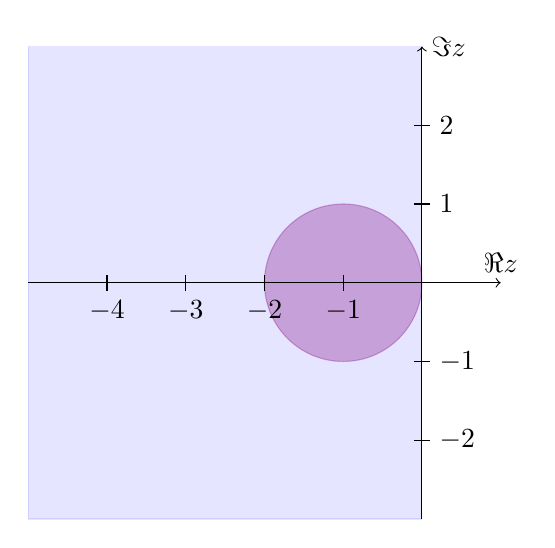
\begin{tikzpicture}
				\filldraw[color = blue, opacity = 0.1] (0,3) -- (0,-3) -- (-5,-3) -- (-5,3) -- cycle;
				\filldraw[color = blue!50!red, opacity = 0.3] (-1,0) circle[radius = 1];
				
				\draw[->] (-5,0) -- (1,0) node [above] {\(\Re z\)};
				\draw[->] (0,-3) -- (0,3) node [right] {\(\Im z\)};
				
				\foreach \x in {-4, ..., -1} {
					\draw (\x, 0.1) -- (\x, -0.1) node [below] {\(\x\)};
				}
				\foreach \x in {-2, -1, 1, 2} {
					\draw (-0.1, \x) -- (0.1, \x) node [right] {\(\x\)};
				}
			\end{tikzpicture}
			
			\caption{Rappresentazione delle regioni di assoluta stabilità dei metodi di Eulero esplicito (in viola), di Eulero implicito e di Crank-Nicolson (in blu).}
		\end{figure}
	\end{esempio}

	\begin{definizione}
		Un metodo numerico è detto \emph{\(A\)-stabile} se la sua regione di assoluta stabilità contiene tutto il semipiano complesso \(\Re z < 0\).
	\end{definizione}

	Dahlquist ha dimostrato le seguenti barriere di stabilità.
	
	\begin{teorema}
		Nessun metodo \inglese{linear multistep} esplicito è \(A\)-stabile.
	\end{teorema}

	\begin{teorema}
		Nessun metodo \inglese{linear multistep} implicito di ordine maggiore di \(2\) è \(A\)-stabile.
	\end{teorema}

\section{Metodi di Runge-Kutta}
	
	\noindent Suddividiamo l'intervallo \([\, x_0, x_{\textup{fin}} \,]\) con punti equispaziati \(x_k = x_0 + k h\) per \(k \in \Set{0, \dots, N_h}\), ove \(h = (x_{\textup{fin}} - x_0) / N_h\); supponiamo che una funzione \(y\) sufficientemente regolare sia la soluzione del problema di Cauchy \eqref{eq:problema-cauchy} in \([\, x_0, x_{\textup{fin}} \,]\) e che la funzione \(f\) che definisce il problema sia continua e \(L\)-lipschitziana nella seconda variabile.
	
	Il metodo numerico di \emph{Runge-Kutta} consiste nel definire una successione \((u_n)_{n \in \N}\) tale che
	\begin{subequations}
		\begin{equation}
			y (x_{n + 1}) \approx u_{n + 1} = u_n + h F (x_n, u_n; h)
		\end{equation}
		ove
		\begin{equation}
			F (x, y; h) = \gamma_1 f (x, y) + \gamma_2 f (x + \alpha h, y + \beta h f (x, y))
		\end{equation}
	\end{subequations}
	Vogliamo determinare \(\gamma_1, \gamma_2, \alpha, \beta\) tali che il metodo sia del secondo ordine, ossia si abbia
	\begin{equation*}
		\tau (h) = \max \Set{\abs{\tau_n (h) : n \in \Set{0, \dots, N_h}}} = \order{h^2}
	\end{equation*}
	ove
	\begin{align*}
		\tau_n (h) &= \frac{y (x_n) - \bar{u}_n}{h} &
		\bar{u}_{n + 1} &= y (x_n) + h F (x_n, y (x_n); h)
	\end{align*}

	\begin{teorema}\label{th:runge-kutta-2}
		Se un metodo di Runge-Kutta è di second'ordine, allora
		\begin{align}
			\gamma_1 + \gamma_2 &= 1 &
			\gamma_2 \alpha &= \frac{1}{2} &
			\gamma_2 \beta &= \frac{1}{2}
		\end{align}
	\end{teorema}

	\begin{esempio}
		Metodi che soddisfano le condizioni del Teorema~\ref{th:runge-kutta-2} sono:
		\begin{itemize}
			\item il metodo di Heun, con \(\alpha = 1\):
			\begin{equation*}
				u_{n + 1} = u_n + \frac{h}{2} \qty[f (x_n, u_n) + f (x_n + h, u_n + h f (x_n, u_n))]
			\end{equation*}
			\item il metodo di Eulero modificato, con \(\alpha = 1 / 2\):
			\begin{equation*}
				u_{n + 1} = u_n + h f \qty(x + \frac{h}{2}, u_n + \frac{h}{2} f (x_n, u_n))
			\end{equation*}
		\end{itemize}
	\end{esempio}

	È possibile calcolare un metodo di Runge-Kutta di ordine \(4\), che è
	\begin{subequations}
		\begin{equation*}
			u_{n + 1} = u_n + h \frac{f_1 + 2 f_2 + 2 f_3 + f_4}{6}
		\end{equation*}
		ove
		\begin{align}
			f_1 &= f (x_n, u_n) \\
			f_2 &= f \qty(x_n + \frac{h}{2}, u_n + \frac{h f_1}{2}) \\
			f_3 &= f \qty(x_n + \frac{h}{2}, u_n + \frac{h f_2}{2}) \\
			f_4 &= f (x_n + h, u_n + h f_3)
		\end{align}
	\end{subequations}